\documentclass[10pt]{beamer}

\usetheme[progressbar=frametitle]{metropolis}
\usepackage{caption}
\usepackage{booktabs}
\usepackage[scale=2]{ccicons}
\usepackage{amsmath}
\usepackage{pgfplots}
\usepgfplotslibrary{dateplot}

\usepackage{xspace}
\newcommand{\themename}{\textbf{\textsc{metropolis}}\xspace}
\definecolor{ODUdark}{HTML}{002B5F}
\definecolor{ODUlight}{HTML}{93BFEB}

\DeclareCaptionFont{tiny}{\tiny}

\setbeamercolor{progress bar}{fg=ODUlight}
\usecolortheme{seahorse}
\setbeamerfont{bibliography entry author}{size=\normalsize,%
                                          series=\normalfont}
\setbeamerfont{bibliography entry title}{size=\normalsize,%
                                         series=\bfseries}
\setbeamerfont{bibliography entry location}{size=\normalsize,%
                                            series=\normalfont}
\setbeamerfont{bibliography entry note}{size=\small,%
                                        series=\normalfont}

\title{CS-834 Intro to Information Retrieval\\First Presentation}
\subtitle{Seminal and Cited Papers}
\date{September 15, 2016}
\author{Plinio H. Vargas}
\institute{Old Dominion University}
\titlegraphic{\hfill
\includegraphics[height=2.5cm]{images/logo}}

\begin{document}

\maketitle
\begin{frame}{Table of Contents}
  \setbeamertemplate{section in toc}[sections numbered]
  \tableofcontents[hideallsubsections]
\end{frame}
%---------------------------------------------
%          Introduction
%---------------------------------------------
\section{Introduction}

\begin{frame}[fragile]{Pre-Google WWW}

  In the beginning there was the \alert{World Wide Web}; and the traffic of knowledge kept increasing, so the number of irrelevant documents recall. Then \alert{Google} was born with the pure notion of using PageRank to bring order to the \textbf{Web}.

\end{frame}
%---------------------------------------------
%          Explaining Google PageRanking
%---------------------------------------------
\section{Google PageRanking}
\begin{frame}{PageRank Calculation}
  \begin{equation*}
	PR(A) = (1-d) + d \left(\frac{PR(T_1)}{C(T_1)} + \cdots + \frac{PR(T_n)}{C(T_n)}\right) \cite{brin1998}
  \end{equation*}
  
  \begin{equation*}
    S(V_i) = (1 - d) + d * \sum_{j\in In(V_i)} \frac{1}{\lvert Out(V_j)\rvert}S(V_j)\cite{mihalcea2004textrank}
  \end{equation*}
\end{frame}
%---------------------------------------------
%          Figure: Three-Web-Pages
%---------------------------------------------
{
\setbeamertemplate{frame footer}{Graph and example taken from textbook\cite{CroftMetzlerStrohman} chapter 4}
\begin{frame}{PageRank Calculation Cont.}
    Internet consisting of only 3 pages. 
  \begin{figure}
		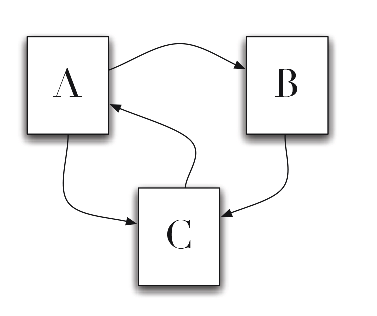
\includegraphics[scale=0.5]{images/Figure1.pdf}
        \caption{Three Web-pages}\label{fig:three-pages}
   \end{figure}
  Since we do not know any of the pages ranking, we will assume that:  
	\begin{equation*}
    	PR(A) = PR(B) = PR(C) = \frac{1}{3} \approx 0.33
	\end{equation*}
\end{frame}

\begin{frame}{PageRank Calculation Cont.}
First iteration:
 	\begin{align*}
    		PR(C) &=\frac{PR(A)}{2}  + \frac{PR(B)}{1}  = \frac{0.33}{2} + \frac{0.33}{1} = 0.5\\
            PR(A) &=\frac{PR(C)}{1}  = \frac{0.33}{1} \approx 0.33\\
            PR(B) &=\frac{PR(A)}{2}  = \frac{0.33}{2} \approx 0.17
	\end{align*}
    
Second iteration:
 	\begin{align*}
    		PR(C) &=\frac{PR(A)}{2}  + \frac{PR(B)}{1}  = \frac{0.33}{2} + \frac{0.17}{1} \approx 0.33\\
            PR(A) &=\frac{PR(C)}{1}  = \frac{0.5}{1} = 0.5\\
            PR(B) &=\frac{PR(A)}{2}  = \frac{0.33}{2} \approx 0.17
	\end{align*}
\end{frame}
}  
{
\setbeamertemplate{frame footer}{See Table \ref{tab:pr-calculation} for full iteration calculation.}
\begin{frame}{PageRank Calculation Cont.}\label{pg:calculation}
Third iteration:
 	\begin{align*}
    		PR(C) &=\frac{PR(A)}{2}  + \frac{PR(B)}{1}  = \frac{0.5}{2} + \frac{0.17}{1} \approx 0.42\\
            PR(A) &=\frac{PR(C)}{1}  = \frac{0.33}{1} \approx 0.33\\
            PR(B) &=\frac{PR(A)}{2}  = \frac{0.5}{2} = 0.25
	\end{align*}
  
After few more iterations:
 	\begin{align*}
    		PR(C) &=\frac{PR(A)}{2}  + \frac{PR(B)}{1}  \approx 0.4\\
            PR(A) &=\frac{PR(C)}{1}  \approx 0.4\\
            PR(B) &=\frac{PR(A)}{2}  \approx 0.2
	\end{align*}
\end{frame}
}
\section{TextRank}

%---------------------------------------------
%          TextRank
%---------------------------------------------
\begin{frame}{TextRank}
A graph-based ranking algorithm of natural language texts with the purpose of:
  \begin{itemize}[<+- | alert@+>]
    \item Keyword Extraction
    \item Sentence Extraction
  \end{itemize}
\end{frame}

%---------------------------------------------
%          TextRank Equation
%---------------------------------------------
\begin{frame}{TextRank Equation}
\alert{TextRank} modified \alert{Google} PageRank “random surfer model” equation:
  \begin{equation}\label{eq:google}
    S(V_i) = (1 - d) + d * \sum_{j\in In(V_i)} \frac{1}{\lvert Out(V_j)\rvert}S(V_j)
  \end{equation}
Taking into account edge 
weights to compute the score associated with
a vertex in the graph:
  \begin{equation}\label{eq:textrank}
    W S(V_i) = (1 - d) + d * \sum\limits_{V_j\in In(V_i)} \frac{w_{ji}}{\sum\limits_{V_k\in Out(V_j)}w_{jk}}W S(V_j)
  \end{equation}  
\end{frame}
%---------------------------------------------
%     TextRank Work Comparison
%---------------------------------------------
\begin{frame}{TextRank Work Comparison}
  Although \alert{TextRank} work is based on equation (\ref{eq:textrank}) taken from \alert{Google} PageRank equation (\ref{eq:google}), its research innovation is in great deal related to A. Hulth \cite{hulth2003improved} “Improved automatic keyword extraction given more linguistic knowledge”.
\end{frame}
%---------------------------------------------
%     Side by Side Comparison
%---------------------------------------------
\begin{frame}{TextRank vs Hulth-2003}
  Comparison between TextRank and Hulth-2003 algorithms:

% Left Column
  \begin{columns}[T,onlytextwidth]
    \column{0.5\textwidth}
    
    \begin{center}
    	TextRank
    \end{center}
    
      \metroset{block=fill}

      \begin{block}{Application}
        Keyword Extraction\\
        Sentence Extraction
      \end{block}

      \begin{alertblock}{Approach}
        Unsupervised
      \end{alertblock}

      \begin{exampleblock}{Example}
        Block content.
      \end{exampleblock}

% Empty space between columns
	\column{0.01\textwidth}

% Right Column
    \column{0.5\textwidth}
    \begin{center}
    	Hulth, 2003
    \end{center}
      \metroset{block=fill}

      \begin{block}{Application}
        Keyword Extraction\\
        Sentence Extraction
      \end{block}

      \begin{alertblock}{Approach}
        Supervised
      \end{alertblock}

      \begin{exampleblock}{Example}
        Block content.
      \end{exampleblock}

  \end{columns}
\end{frame}
%---------------------------------------------
%          TextRank Keyword Extraction Example
%---------------------------------------------
{
\setbeamertemplate{frame footer}{Source: \cite{mihalcea2004textrank}}
\begin{frame}{TextRank Keyword Extraction Example}
\begin{figure}\caption{Keywords Extraction Graph Example}
	\center
	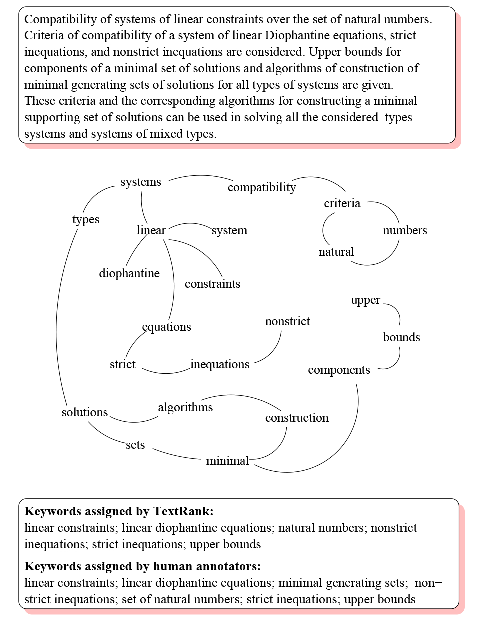
\includegraphics[scale=0.5]{images/mihalcea_pg4.pdf}
\end{figure} 
\begin{center}
\tiny Sample graph built for keyphrase extraction from an Inspec abstract.
\end{center}
\end{frame}
}
%---------------------------------------------
%          TextRank Steps
%---------------------------------------------
\begin{frame}{TextRank Steps}
  \begin{enumerate}[<+- | alert@+>]
    \item Text is tokenized
    \item Edge is added between lexical units
    \item Each vertex is set to initial value of 1
    \item TextRank algorithm runs until it converges
  \end{enumerate}
\end{frame}
%---------------------------------------------
%          Conclusion
%---------------------------------------------
\section{Conclusion}

\begin{frame}{Summary}
\begin{center}Working on it.\end{center}
\end{frame}

\begin{frame}[standout]
  Questions?
\end{frame}

\appendix
%---------------------------------------------
%     Table for Figure with Three-Web-Pages
%---------------------------------------------
\begin{frame}[fragile]{Tables}
\begin{table}
\begin{center}
\tiny
\caption{PageRank Iteration Calculation for Figure \ref{fig:three-pages}}\label{tab:pr-calculation}
\begin{tabular}{c c c c c c c}
\toprule
Iteration & A &	B & C & A-Error & B-Error & C-Error\\
\midrule
0 & 0.333333 & 0.333333 & 0.333333 & - & - & -\\
1 & 0.333333 & 0.500000 & 0.166667 & 0.0000 & 0.1667 & 0.1667\\
2 & 0.500000 & 0.333333 & 0.166667 & 0.1667 & 0.1667 & 0.0000\\
3 & 0.333333 & 0.416667 & 0.250000 & 0.1667 & 0.0833 & 0.0833\\
4 & 0.416667 & 0.416667 & 0.166667 & 0.0833 & 0.0000 & 0.0833\\
5 & 0.416667 & 0.375000 & 0.208333 & 0.0000 & 0.0417 & 0.0417\\
6 & 0.375000 & 0.416667 & 0.208333 & 0.0417 & 0.0417 & 0.0000\\
7 & 0.416667 & 0.395833 & 0.187500 & 0.0417 & 0.0208 & 0.0208\\
8 & 0.395833 & 0.395833 & 0.208333 & 0.0208 & 0.0000 & 0.0208\\
9 & 0.395833 & 0.406250 & 0.197917 & 0.0000 & 0.0104 & 0.0104\\
10 & 0.406250 & 0.395833 & 0.197917 & 0.0104 & 0.0104 & 0.0000\\
11 & 0.395833 & 0.401042 & 0.203125 & 0.0104 & 0.0052 & 0.0052\\
12 & 0.401042 & 0.401042 & 0.197917 & 0.0052 & 0.0000 & 0.0052\\
13 & 0.401042 & 0.398438 & 0.200521 & 0.0000 & 0.0026 & 0.0026\\
14 & 0.398438 & 0.401042 & 0.200521 & 0.0026 & 0.0026 & 0.0000\\
15 & 0.401042 & 0.399740 & 0.199219 & 0.0026 & 0.0013 & 0.0013\\
16 & 0.399740 & 0.399740 & 0.200521 & 0.0013 & 0.0000 & 0.0013\\
17 & 0.399740 & 0.400391 & 0.199870 & 0.0000 & 0.0007 & 0.0007\\
18 & 0.400391 & 0.399740 & 0.199870 & 0.0007 & 0.0007 & 0.0000\\
19 & 0.399740 & 0.400065 & 0.200195 & 0.0007 & 0.0003 & 0.0003\\
20 & 0.400065 & 0.400065 & 0.199870 & 0.0003 & 0.0000 & 0.0003\\
21 & 0.400065 & 0.399902 & 0.200033 & 0.0000 & 0.0002 & 0.0002\\
22 & 0.399902 & 0.400065 & 0.200033 & 0.0002 & 0.0002 & 0.0000\\
23 & 0.400065 & 0.399984 & 0.199951 & 0.0002 & 0.0001 & 0.0001\\
24 & 0.399984 & 0.399984 & 0.200033 & 0.0001 & 0.0000 & 0.0001\\
\bottomrule
\end{tabular}
\end{center}
\end{table}
\begin{center}
	\tiny
    \vspace{-5mm}
    Final result is shown on page \ref{pg:calculation}
\end{center}
\end{frame}
%---------------------------------------------
%     Table for Figure with Three-Web-Pages
%---------------------------------------------
\begin{frame}[fragile]{Keyword Extraction Results}
\begin{table}
\begin{center}
\tiny
\label{tab:hulth}
\caption{\tiny Results for automatic keyword extraction using TextRank or supervised learning (Hulth, 2003)}
\begin{tabular}{l c c c c c c c}
\toprule
& \multicolumn{2}{c}{Assigned} & \multicolumn{2}{c}{Correct}\\
\cline{2-5}
Method & Total & Mean & Total & Mean & Precision & Recall & F-measure\\
\midrule
\\
TextRank\\
\hline
Undirected, Co-occ.window=2 & 6,784 & 13.7 & 2,116 & 4.2 & \emph{\textbf{31.2}} & 43.1 & \emph{\textbf{36.2}}\\
Undirected, Co-occ.window=3 & 6,715 & 13.4 & 1,897 & 3.8 & 28.2 & 38.6 & 32.6\\
Undirected, Co-occ.window=5 & 6,558 & 13.1 & 1,851 & 3.7 & 28.2 & 37.7 & 32.2\\
Undirected, Co-occ.window=10 & 6,570 & 13.1 & 1,846 & 3.7 & 28.1 & 37.6 & 32.2\\
Directed, forward, Co-occ.window=2 & 6,662 & 13.3 & 2,081 & 4.1 & 31.2 & 42.3 & 35.9\\
Directed, backward, Co-occ.window=2 & 6,636 & 13.3 & 2,082 & 4.1 & 31.2 & 42.3 & 35.9\\
\\
Hulth (2003)\\
\hline
Ngram with tag & 7,815 & 15.6 & 1,973 & 3.9 & 25.2 & \emph{\textbf{51.7}} & 33.9\\
NP-chunks with tag & 4,788 & 9.6 & 1,421 & 2.8 & 29.7 & 37.2 & 33.0\\
Pattern with tag & 7,012 & 14.0 & 1,523 & 3.1 & 21.7 & 39.9 & 28.1\\
\bottomrule
\end{tabular}
\end{center}
\end{table}
\end{frame}
%\begin{frame}[fragile]{Backup slides}
%  Sometimes, it is useful to add slides at the end of your presentation to
%  refer to during audience questions.
%
%  The best way to do this is to include the \verb|appendixnumberbeamer|
%  package in your preamble and call \verb|\appendix| before your backup slides.
%
%  \themename will automatically turn off slide numbering and progress bars for
%  slides in the appendix.
%\end{frame}

\begin{frame}[allowframebreaks]{References}

  \bibliography{demo}
  %styles{ieeetr, plain, abbrv, acm, unsrt, alpha, apalike, siam}
  \bibliographystyle{siam}

\end{frame}

\end{document}